\scanpage{17}
\uline{Cas particuliers}

Supposons que $\forall i\in I$, \deleted{$E_i$ \unsure{est|soit} rare dans $X$.} \inserted{on ait} (si $\Sigma_i^+\ \Sigma_i^-$ sont les deux comp. conn. de $X\setminus\Sigma_i$)

\deleted{Alors on trouve que}
\[
\begin{aligned}
\overline{\Sigma_i^+} &= \Sigma_i^+\cup E_i\\
\overline{\Sigma_i^-} &= \Sigma_i^-\cup E_i .
\end{aligned}
\]

Alors je dis qu'on a
\[
\overline{\Sigma_{12}}=\Sigma_{12}
% G01: retraced cup; full-scan origin (944,783), fixed local rectangle 36 by 36.
\mathbin{\vcenter{\hbox{
\begin{tikzpicture}[x=0.007cm,y=-0.007cm,baseline=0pt]
\path[use as bounding box] (0,0) rectangle (36,36);
\draw[line width=0.55pt,line cap=round,line join=round] (7,5) .. controls (7,13) and (7,21) .. (9,25) .. controls (18,33) and (32,30) .. (32,14) -- (30,7);
\draw[line width=0.4pt,line cap=round,line join=round] (25,7) .. controls (32,20) and (20,32) .. (8,25);
\end{tikzpicture}}}} E_1\cup E_2
\]

% G02: short curved separator with downturned right endpoint.
% Full-scan origin (300,887); fixed local rectangle 240 by 22.
\figure{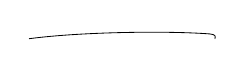
\begin{tikzpicture}[x=0.01cm,y=-0.01cm,baseline=0pt]
\path[use as bounding box] (0,0) rectangle (240,22);
\draw[line width=0.3pt,line cap=round] (2,14) .. controls (70,5) and (181,4) .. (232,8) .. controls (238,9) and (239,10) .. (238,14);
\end{tikzpicture}}

% slanted
\reversemarginpar
\margin{introduire la partition $\unsure{\Pi|\pi}_j=\{\deleted{\unsure{\Sigma}}E_j,\Sigma_j^+,\Sigma_j^-\}$}
\normalmarginpar
\deleted{Supposons}

Soit $J\subset I$ tel que $I=J\amalg\{i\}$.

Considerons la partition
% G03: upper Pi_J insertion and curved guide. Source origin (1215,1100).
% Fixed rectangle 175 by 135; base-west anchors and zero node separations.
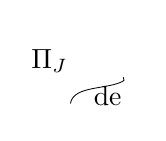
\begin{tikzpicture}[x=0.008cm,y=-0.008cm,baseline=(pide.base)]
\path[use as bounding box] (0,0) rectangle (175,135);
\node[anchor=base west,inner sep=0pt,outer sep=0pt] at (6,65) {\inserted{$\Pi_J$}};
\node[anchor=base west,inner sep=0pt,outer sep=0pt] (pide) at (105,124) {de};
\draw[line width=0.3pt,line cap=round] (68,120) .. controls (73,91) and (129,99) .. (153,84) -- (152,79);
\end{tikzpicture}
$X$ \deleted{definie} definie par les $\deleted{\Sigma}E_j$ $(j\in J)$, \deleted{et} \unsure{Intersection|intersection} des partitions
% G04: ternaires Pi_j insertion and its long bent caret. Source origin (970,1345).
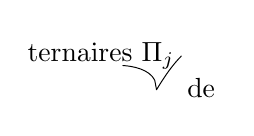
\begin{tikzpicture}[x=0.0075cm,y=-0.0075cm,baseline=(terde.base)]
\path[use as bounding box] (0,0) rectangle (335,135);
\node[anchor=base west,inner sep=0pt,outer sep=0pt] at (0,57) {\inserted{ternaires $\Pi_j$}};
\node[anchor=base west,inner sep=0pt,outer sep=0pt] (terde) at (270,118) {de};
\draw[line width=0.35pt,line cap=round,line join=round] (161,64) .. controls (177,65) and (206,70) .. (215,89) -- (218,105) .. controls (233,80) and (246,62) .. (260,48);
\end{tikzpicture}
$X$ $(j\in J)$ definies par les $E_j$ \deleted{$\unsure{\in|E}$} $(j\in J)$
\[
X=E_j\amalg\coprod_{\alpha\in\pi_0(X\setminus E_j)}\Sigma_j^{\unsure{\prime|\cdot}\alpha}
\]
% G05 is the small detached oblique mark immediately before upper alpha.
% It is represented once by the qualified prime/dot candidate above; no role is assigned.

% G11: two detached marks at far right between display and lower prose.
% Full-scan origin (1567,1735), fixed local rectangle 18 by 20.
% Shapes only: character, role, hand and surface origin remain unestablished.
\margin{\unsure{\begin{tikzpicture}[x=0.02cm,y=-0.02cm,baseline=0pt]
\path[use as bounding box] (0,0) rectangle (18,20);
\fill (9,5) .. controls (11,4) and (13,6) .. (11,9) .. controls (8,10) and (8,7) .. cycle;
\fill (4,12) .. controls (7,11) and (8,14) .. (5,15) .. controls (3,16) and (2,13) .. cycle;
\end{tikzpicture}}}

-- c'est aussi la partition definie par celle de $\displaystyle\unsure{.}\,\bigcup_{j\in J}E_j$ en les $E_j$, et la partition
% G06 is the detached baseline point before the first indexed union, represented once above.
% G07: lower Pi_J insertion and curved guide. Source origin (770,1965).
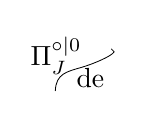
\begin{tikzpicture}[x=0.009cm,y=-0.009cm,baseline=(lowde.base)]
\path[use as bounding box] (0,0) rectangle (145,100);
\node[anchor=base west,inner sep=0pt,outer sep=0pt] at (4,54) {\inserted{$\Pi_J^{\unsure{\circ|0}}$}};
\node[anchor=base west,inner sep=0pt,outer sep=0pt] (lowde) at (69,85) {de};
\draw[line width=0.3pt,line cap=round] (39,89) .. controls (40,65) and (55,62) .. (76,56) .. controls (93,51) and (119,40) .. (122,34) -- (118,30);
\end{tikzpicture}
$\displaystyle X\setminus
% G08: union with visible transverse stroke; interpretation of stroke stays qualified.
% Full-scan origin (1115,1970), fixed local rectangle 80 by 75.
\mathop{\unsure{\vcenter{\hbox{
\begin{tikzpicture}[x=0.009cm,y=-0.009cm,baseline=0pt]
\path[use as bounding box] (0,0) rectangle (80,75);
\draw[line width=0.45pt,line cap=round] (18,9) .. controls (13,34) and (18,60) .. (38,63) .. controls (61,67) and (70,39) .. (63,10);
\draw[line width=0.4pt,line cap=round] (12,20) .. controls (26,20) and (39,17) .. (59,18);
\end{tikzpicture}}}}}\limits_{j\in J}E_j$
intersection des partitions binaires $\Pi_{J,j}^{\circ}$
% G09: inserted quantifier and guide over induites. Source origin (1230,2070).
% The recurring circle/zero doubt is marked at its first occurrence above.

\begin{tikzpicture}[x=0.0075cm,y=-0.0075cm,baseline=(induites.base)]
\path[use as bounding box] (0,0) rectangle (335,115);
\node[anchor=base west,inner sep=0pt,outer sep=0pt] at (60,45) {\inserted{$(j\in J)$}};
\node[anchor=base west,inner sep=0pt,outer sep=0pt] (induites) at (52,91) {induites};
\draw[line width=0.3pt,line cap=round] (14,92) .. controls (0,72) and (30,57) .. (53,53) .. controls (99,66) and (189,54) .. (219,41) .. controls (224,39) and (216,32) .. (214,31);
\end{tikzpicture}
% G10: inserted U_J= and guide curling down to the right of sur.
% Full-scan origin (320,2155); fixed local rectangle 145 by 155.
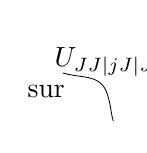
\begin{tikzpicture}[x=0.008cm,y=-0.008cm,baseline=(sur.base)]
\path[use as bounding box] (0,0) rectangle (145,155);
\node[anchor=base west,inner sep=0pt,outer sep=0pt] at (43,61) {\inserted{$U_{\unsure{\deleted{J}J|\deleted{j}J|J}}={}$}};
\node[anchor=base west,inner sep=0pt,outer sep=0pt] (sur) at (0,111) {sur};
\draw[line width=0.3pt,line cap=round] (56,72) .. controls (88,81) and (111,74) .. (124,99) .. controls (133,121) and (132,138) .. (136,148);
\end{tikzpicture}
$\displaystyle X\setminus\bigcup_{j\in J}E_j$ par les $\Pi_j$ $(\unsure{g|j}\in J)$. Pour
% archive sheet number: 16
